\documentclass{beamer}
\usetheme{sintef}

\usefonttheme{serif}
\usepackage{amsmath,amsthm,amssymb,amsfonts,oldgerm}
\usepackage[T1]{fontenc}
\usepackage{mathpazo}
\usepackage{xmpmulti}

\newcommand{\testcolor}[2]{\colorbox{#1}{#2}}

\titlebackground*{images/background}

\title{Clasificación de los dígitos escritos en los telegramas de las elecciones legislativas en Santa Fe mediante técnicas de adaptación de dominio.}
\course{Maestría en Explotación de Datos y Gestión del Conocimiento}
\author{Franco \textsc{Lianza}}

\begin{document}
\maketitle

\section{Introducción}

\section{Marco Teórico}

\subsection{Adaptación de Dominio}

\begin{frame}{Qué causa un mal rendimiento?}
      \begin{columns}
            \begin{column}{0.55\textwidth}
                  \begin{itemize}
                        \item Los conjuntos de datos provienen de distribuciones diferentes.
                        \item El modelo no aprende características comunes en los datos.
                  \end{itemize}
            \end{column}
            \begin{column}{0.4\textwidth}
                  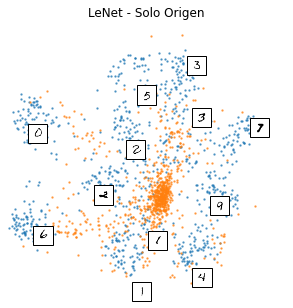
\includegraphics[width=\textwidth]{images/marco-teorico/umap-lenet-so.png}
            \end{column}
      \end{columns}
\end{frame}

\begin{frame}{Algunas soluciones}
      \begin{columns}
            \begin{column}{0.55\textwidth}
                  \begin{itemize}
                        \item Utilizar un modelo más potente.
                        \item Data augmentation.
                        \item Métodos de entrenamiento semi-supervisados.
                        \item Recolectar más datos.
                        \item \testcolor{sintefgreen}{Adaptación de dominio.}
                  \end{itemize}
            \end{column}
            \begin{column}{0.4\textwidth}
                  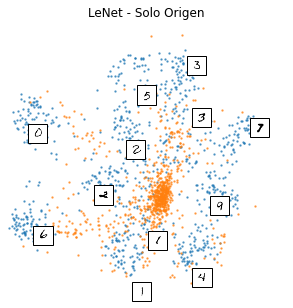
\includegraphics[width=\textwidth]{images/marco-teorico/umap-lenet-so.png}
            \end{column}
      \end{columns}
\end{frame}

\begin{frame}{Adaptación de dominio}
      \begin{columns}
            \begin{column}{0.4\textwidth}
                  \begin{colorblock}[black]{white}{Dominio origen}
                        \centering
                        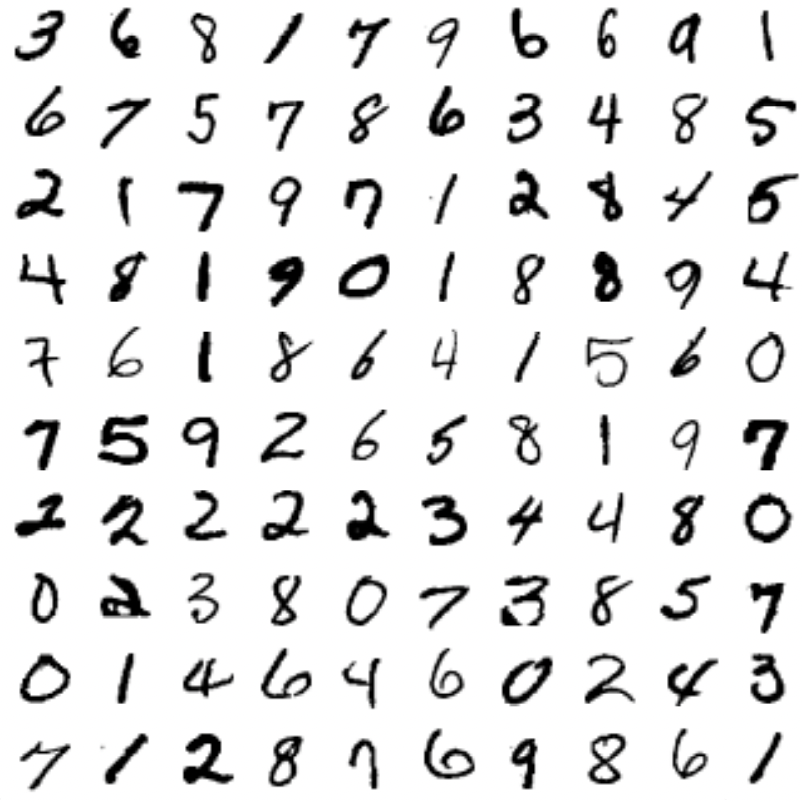
\includegraphics[width=0.5\textwidth]{images/marco-teorico/mnist.png}
                  \end{colorblock}
            \end{column}
            \begin{column}{0.15\textwidth}
                  \centering
                  $\nLeftrightarrow$
            \end{column}
            \begin{column}{0.4\textwidth}
                  \begin{colorblock}[black]{white}{Dominio destino}
                        \centering
                        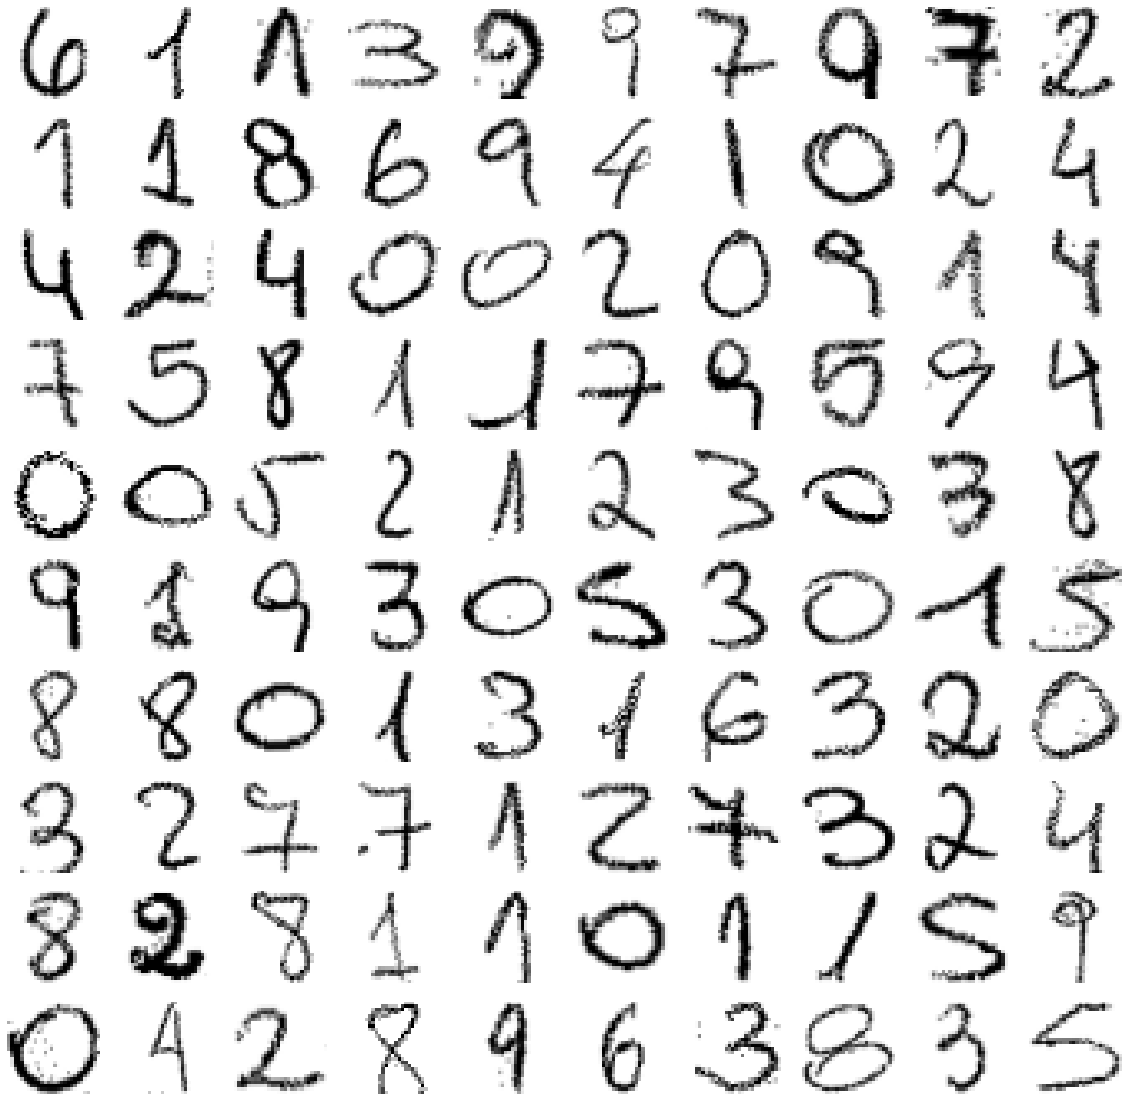
\includegraphics[width=0.5\textwidth]{images/marco-teorico/tds.png}
                  \end{colorblock}
            \end{column}
      \end{columns}
      \vfill
      \begin{itemize}
            \item Sabemos las etiquetas del dominio origen y no sabemos las de destino.
            \item Vemos los datos de destino.
      \end{itemize}
\end{frame}

\begin{frame}{Alineación de dominios}
      \multiinclude[format=jpg,start=1,graphics={width=\textwidth}]{images/marco-teorico/alineacion/alineacion-dominios}
\end{frame}

\subsection{Algo2}

\section{Metodología}
\section{Análisis de Resultados}
\section{Conclusiones}

\backmatter
\end{document}
